\documentclass[oneside, 11pt]{article}

\usepackage[T1]{fontenc}
\usepackage[utf8]{inputenc}
\usepackage[english]{babel}

\usepackage{fouriernc}
\usepackage[detect-all, binary-units, separate-uncertainty=true,
            per-mode=symbol, retain-explicit-plus, retain-unity-mantissa=false]{siunitx}

\usepackage{setspace}
\setstretch{1.2}

\setlength{\parskip}{\smallskipamount}
\setlength{\parindent}{0pt}

\usepackage[headheight=14pt]{geometry}
\geometry{marginparwidth=0.5cm, verbose, a4paper, tmargin=3cm, bmargin=3cm,
          lmargin=2cm, rmargin=2cm}

\usepackage{float}

\usepackage[fleqn]{amsmath}
\numberwithin{equation}{section}
\numberwithin{figure}{section}

\usepackage{graphicx}
\graphicspath{{images/}{../../../images/}}

\usepackage{tikz}
\usetikzlibrary{shapes}
\usetikzlibrary{plotmarks}

\newcounter{Exercise}
\setcounter{Exercise}{1}
\usepackage{xcolor}
\definecolor{shadecolor}{gray}{0.9}
\usepackage{framed}
\usepackage{caption}

\usepackage{url}


\usepackage{fancyhdr}
\pagestyle{fancy}
\fancyhf{}
\rhead{\thepage}
\renewcommand{\footrulewidth}{0pt}
\renewcommand{\headrulewidth}{0pt}

\fancypagestyle{firststyle}
{
    \fancyhf{}
    \rhead{\thepage}
    \cfoot{
\includegraphics[height=30pt]{HiSPARClogo}}
    \rfoot{
\includegraphics[height=25pt]{CCbysa}}
    \lfoot{
\includegraphics[height=30pt]{NIKHEFlogo}}
    \renewcommand{\footskip}{50pt}
    \renewcommand{\footrulewidth}{0.1pt}
    \renewcommand{\headrulewidth}{0pt}
}

\newcommand{\figref}[1]{Figuur~\ref{#1}}

\newcommand{\hisparc}{\textsmaller{HiSPARC}\xspace}
\newcommand{\kascade}{\textsmaller{KASCADE}\xspace}
\newcommand{\sapphire}{\textsmaller{SAPPHiRE}\xspace}
\newcommand{\jsparc}{\textsmaller{jSparc}\xspace}
\newcommand{\hdf}{\textsmaller{HDF5}\xspace}
\newcommand{\aires}{\textsmaller{AIRES}\xspace}
\newcommand{\csv}{\textsmaller{CSV}\xspace}
\newcommand{\python}{\textsmaller{PYTHON}\xspace}
\newcommand{\corsika}{\textsmaller{CORSIKA}\xspace}
\newcommand{\labview}{\textsmaller{LabVIEW}\xspace}
\newcommand{\daq}{\textsmaller{DAQ}\xspace}
\newcommand{\adc}{\textsmaller{ADC}\xspace}
\newcommand{\hi}{\textsc{h i}\xspace}
\newcommand{\hii}{\textsc{h ii}\xspace}
\newcommand{\mip}{\textsmaller{MIP}\xspace}
\newcommand{\hisparcii}{\textsmaller{HiSPARC II}\xspace}
\newcommand{\hisparciii}{\textsmaller{HiSPARC III}\xspace}

\DeclareSIUnit{\electronvolt}{\ensuremath{\mathrm{e\!\!\:V}}}

\DeclareSIUnit{\unitsigma}{\ensuremath{\sigma}}
\DeclareSIUnit{\mip}{\textsmaller{MIP}}
\DeclareSIUnit{\adc}{\textsmaller{ADC}}

\DeclareSIUnit{\gauss}{G}
\DeclareSIUnit{\parsec}{pc}
\DeclareSIUnit{\year}{yr}



\begin{document}

\title{De Hemel}
\author{N.G. Schultheiss}
\date{}

\maketitle
\thispagestyle{firststyle}

\section{Inleiding}

Deze module is direct te volgen vanaf de derde klas. Deze module wordt
vervolgd met de module ``Het heelal''. Uiteindelijk kun je met de
opgedane kennis een telescoop als meetinstrument toepassen. 


\section{Hoeken}

\begin{figure}[H]
\noindent \begin{centering}
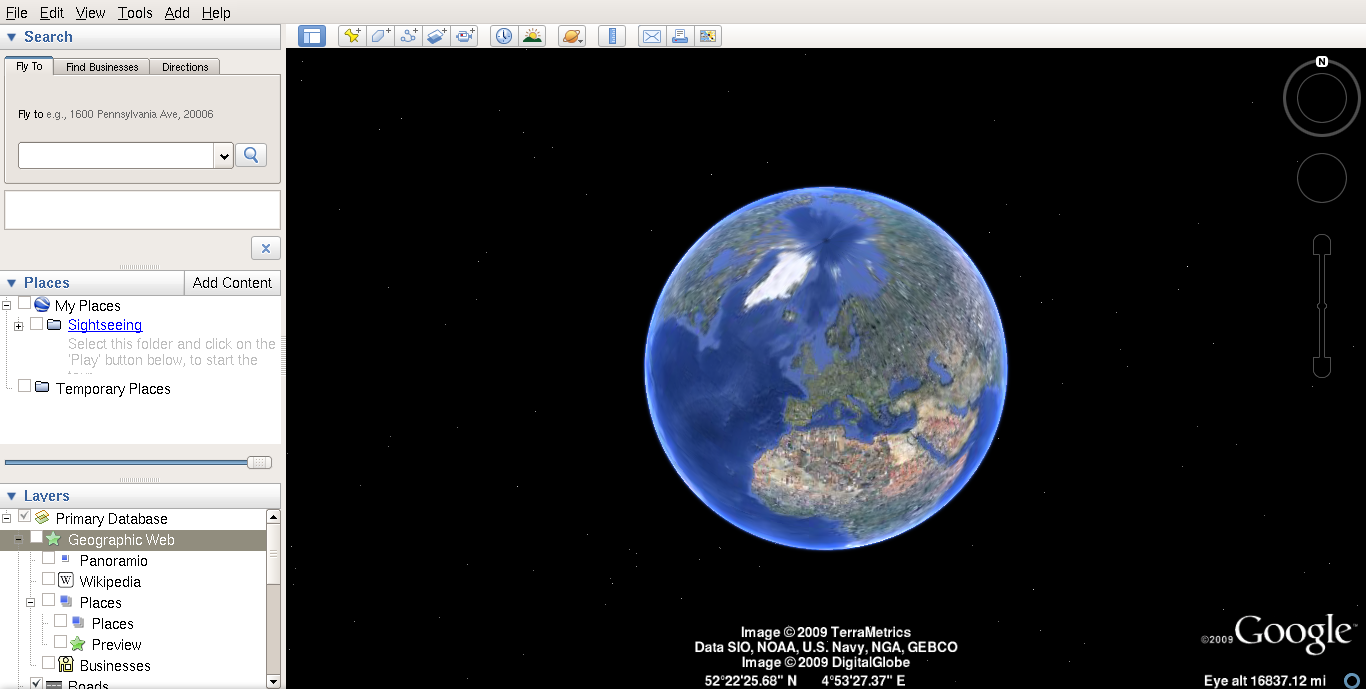
\includegraphics[width=16cm]{Screenshot-Google-Earth}
\par\end{centering}

\caption{De Aarde met Google-Earth}
\end{figure}


Op Google-Earth zie je onder in het scherm $52^{o}22'23.38"N$ en
$4^{o}53'35.84"E$ \footnote{In Nederland gebruikt men een komma (,) na
de eenheden en voor de tienden. In de meeste landen gebruikt men
inplaats van de komma een punt (.).} als je de Dam in Amsterdam
aanwijst. Het aantal graden (52) is hier direct in te herkennen.
Daarnaast staat $22'$, of in spreektaal 22 (boog-)minuten. Net als bij
de tijd waar 1 uur in 60 minuten wordt verdeeld, kun je 1 graad ook in
60 (boog-)minuten verdelen. Daarnaast zie je $23.38"$, of 23.38
(boog-)seconden, 1 (boog-)minuut is natuurlijk 60 (boog-)seconden. Op
deze manier kunnen we dus heel nauwkeurig een plaats met hoeken
vastleggen. 

Rond de Aarde lopen cirkels over de Noordpool en de Zuidpool, de helft
van deze cirkel (van Noordpool naar Zuidpool) noemen we een meridiaan.
Bij de Noordpool (en de Zuidpool) maken de meridianen hoeken met elkaar. 

Per definitie loopt de $0^{o}$ meridiaan door the Royal Observatory
in Greenwich, een wijk van London. De hoek tussen de meridiaan door
Greenwich en de meridiaan door de Dam is dus $4^{o}53'35.84"$ naar
het Oosten of OosterLengte. Ga je vanaf de evenaar langs de meridiaan
omhoog dan doorloop je een hoek van $52^{o}22'23.38"$ naar het Noorden
of NoorderBreedte. We hebben nu een manier om plaatsen op Aarde aan
te wijzen.

Een hoek met graden, boogminuten en boogseconden is om te zetten in
een hoek met alleen graden en cijfers achter de komma:

\[
4^{o}53'35,84"=4^{o}+\left(\frac{53}{60}\right)^{o}+\left(\frac{35,84}{3600}\right)^{o}
=\left(4+0,883333+0,009956\right)^{o}=4,893289^{o}
\]


Een hoek met graden en cijfers achter de komma is natuurlijk ook om
te zetten in een hoek met graden, boogminuten en boogseconden:

\[
13,236782^{o}=13^{o}+0,236782^{o}
\]


\[
13^{o}+0,236782^{o}=13^{o}+60*0,236782'=13^{o}14'+0,20692'
\]


\[
13^{o}14'+0,20692'=13^{o}14'+60*0,20692"=13^{o}14'12,42"
\]


\paragraph*{Opdracht 1:}

\emph{Een hoek is gemeten als $24,7381^{0}$. Bereken hoeveel graden,
boogminuten en boogseconden dit is.}


\paragraph*{Opdracht 2:}

\emph{Een hoek is gemeten als $52^{o}23'17"$. Bereken de hoek met
cijfers achter de komma.}


\section{De hemel}

Boven in het venster van Google-Earth zie je een ``Saturnus'' icoontje.
Als je hier op klikt zie je de sterren aan de hemel.

\begin{figure}[H]
\noindent \begin{centering}
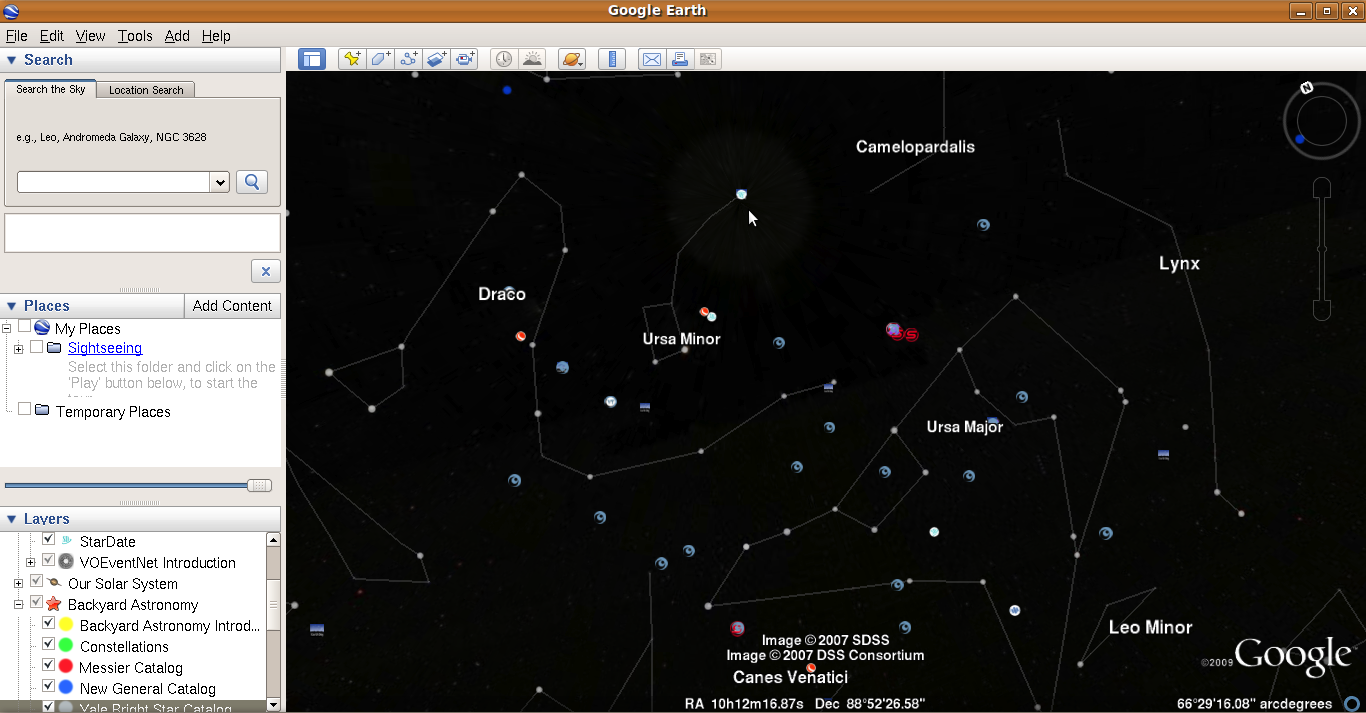
\includegraphics[width=16cm]{Screenshot-Google-Earth-Stars}
\par\end{centering}

\caption{De hemel met Google-Earth}
\end{figure}


In figuur 2.2 zijn de sterren aan de Noordelijke hemel te zien. De
muis wijst naar de poolster. Onder in het scherm is RA 10h12m16.87s
en Dec $88^{o}52'26.58"$ te zien. 

De afkorting RA staat voor ``Right Ascension'' of in het Nederlands
``Rechte Klimming'' (RK). De Rechte Klimming van de hemel is te
vergelijken met de (Ooster- of Wester-)Lengte op Aarde. De Rechte
Klimming geeft dus een soort hemel-meridiaan aan.

Als je de hemel-meridiaan over een bepaalde hoek volgt krijg je de
Declinatie. Op Aarde kennen we een (Noorder- of Zuider-)Breedte, in
de hemel is de Breedte te vergelijken met de Declinatie. 

Dit kan niet vanaf de Evenaar want deze is op Aarde. Als een hemelobject,
zoals een ster of planeet, in het vlak door de evenaar ligt, zien
we dit op Aarde op de Hemelequator. Soms ligt een object boven of
beneden de Hemelequator. Het objevt heeft dan een Declinatie. Deze
wordt vanaf de Hemelequator gemeten.

Omdat de Aardas schuin staat ten opzichte van de Zon, beweegt de Zon
niet langs de Hemelequator. De Zon beweegt langs een cirkel die schuin
staat ten opzichte van de Hemelequator. Deze cirkel noemen we de Ecliptica.
De Ecliptica snijdt de Hemelequator twee maal, bij het Lentepunt en
bij het Herfstpunt. De ``Hemel-meridianen'' worden gemeten vanaf
het Lentepunt.


\paragraph*{Opdracht 3:}

\emph{Ga in Google-Earth in de hemel naar een rechte klimming van
0h0m0s} \footnote{Ik volg hier de notatie van Google-earth. Meestal
wordt de 0h0m0s opgeschreven als 0:0:0.}\emph{ en een declinatie van
$0^{o}0'0"$. In welk sterrenbeeld / bij welk sterrenbeeld ligt dit punt?
}


\paragraph*{Opdracht 4:}

\emph{Ga in Google-Earth in de hemel naar een rechte klimming van
2h0m0s en een declinatie van $0^{o}0'0"$. In welk sterrenbeeld /
bij welk sterrenbeeld van de dierenriem ligt dit punt? Herhaal dit
voor 4h0m0s, 6h0m0s, 8h0m0s, 10h0m0s, 12h0m0s, 14h0m0s, 16h0m0s, 18h0m0s,
20h0m0s en 22h0m0s. Zet de namen van de sterrenbeelden in een tabel.
Let op: De Declinatie is voor sterrenbeelden van de dierenriem niet
altijd $0^{o}0'0"$! De cirkel is rond bij 24h0m0s.}

Aan het begin van de lente staat de zon in het sterrenbeeld ``Vissen''.
Dit klopt omdat de tijd begint te lopen vanaf het lentepunt
\footnote{Volgens de Astrologie is het lentepunt in het sterrenbeeld
Ram. In de afgelopen 2000 jaar is de Aardas verdraaid en wijst deze naar
een andere plaats aan de hemel. Het Lentepunt is daarom naar ``Vissen''
geschoven.}. Dit is overigens niet de normale Aardtijd die ten opzichte
van de Zon wordt gemeten. Deze tijd is de tijd die ten opzichte van de
sterren / sterrenbeelden wordt gemeten, een soort hemelse tijd of
``Siderische tijd''.


\paragraph*{Opdracht 5:}

Maak de onderstaande tabel af:

\noindent \begin{flushleft}
\begin{tabular}{|>{\centering}p{5cm}|>{\centering}p{5cm}|}
\hline 
Aarde & Hemel\tabularnewline
\hline 
\hline 
Lengte & \tabularnewline
\hline 
 & Declinatie\tabularnewline
\hline 
Evenaar & \tabularnewline
\hline 
\end{tabular}
\par\end{flushleft}


\section{Herschel en Messier}

Fredrich Wilhelm Herschel verdiende zijn geld als muzikant en schreef
onder andere verschillende symphoniën. Hij had echter ook een grote
interesse in de hemel en bouwde daarom verschillende refractors waarmee
hij de hemel bestudeerde.

Ongeveer tegelijkertijd onderzocht Charles Messier de hemel. Hij maakte
een catalogus met 110 Messier objecten. Deze zijn nog steeds bekend
als M001 tot en met M110. Herschel was onder de indruk van het werk
van Messier en maakte zelf een catalogus van 2514 objecten in de verre
ruimte.

\begin{figure}[h]
\begin{verbatim}
Name       Type          R.A.     Dec     Size  Mag   Con  Herschel
 AR   37   Open cluster  11:32.5  +74~32              Dra  H969-3
 IC  434   Nebula         5:41.0  - 2~24  60.0        Ori  H35-5 Barnard’s Loop
 IC 2995   Galaxy        12:05.8  -27~56   3.1  13.5  Hya  H382-3
 IC 4051   Galaxy        13:00.9  +28~00   1.1  13.2  Com  H363-3
NGC   12   Galaxy         0:08.7  + 4~37   1.9  14.1  Psc  H868-3
NGC   13   Galaxy         0:08.8  +33~26   2.7  13.6  And  H866-3
NGC   14   Galaxy         0:08.8  +15~49   3.0  12.1  Peg  H591-2
NGC   16   Galaxy         0:09.1  +27~44   2.1  12.0  Peg  H15-4 vF interacting pair
NGC   23   Galaxy         0:09.9  +25~55   2.3  12.0  Peg  H147-3
NGC   24   Galaxy         0:09.9  -24~58   5.5  11.5  Scl  H461-3 Nearly edge-on
NGC   29   Galaxy         0:10.8  +33~21   1.8  12.6  And  H853-2
NGC   36   Galaxy         0:11.4  + 6~23   2.4  14.4  Psc  H456-3
NGC   39   Galaxy         0:12.3  +31~03   1.1  13.5  And  H861-3
NGC   40   Planetary neb  0:13.0  +72~32    .3  10.7  Cep  H58-4 "400"
NGC   52   Galaxy         0:14.6  +18~33   2.4  13.3  Peg  H183-3
NGC   57   Galaxy         0:15.4  +17~18   2.6  11.6  Psc  H241-2 = H243-2
NGC   61A  Galaxy         0:16.5  - 6~14   1.1  14.7  Psc  H428-3
NGC   68   Galaxy         0:18.3  +30~04   1.5  13.0  And  H16-5
NGC   95   Galaxy         0:22.2  +10~30   1.9  12.6  Psc  H257-2 asym uneven arms
\end{verbatim}
\caption{Een klein deel van de Herschel catalogus}
\end{figure}


\paragraph*{Opdracht 5:}

\emph{Kijk of je deze objecten met Google-Earth kunt vinden. Als we
naar ``AR 37 / H969-3'' kijken, heeft dit object een rechte klimming
van} 11:32.5 \emph{of} 11h32,5m (11h32m30s) \emph{en een declinatie
van} +74~32 \emph{of }$74^{o}32'$.

\begin{figure}[h]
\noindent \begin{centering}
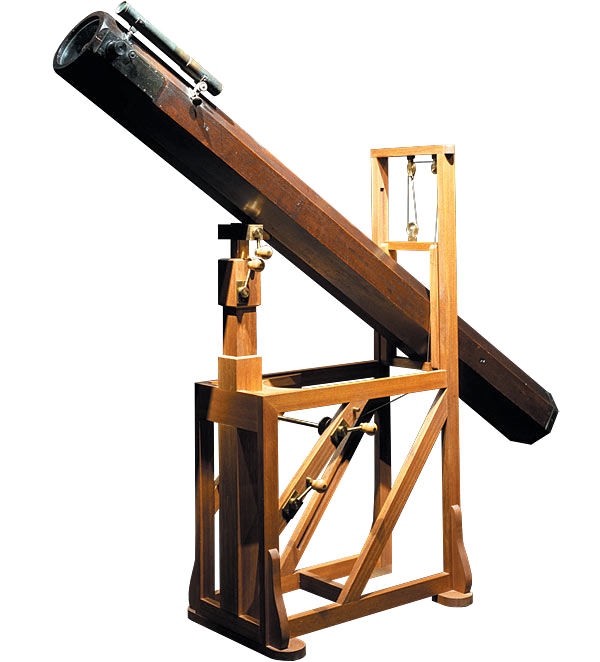
\includegraphics[width=8cm]{herschel_small_telescope}
\par\end{centering}

\caption{De eerste telescoop van Herschel\cite{herschel}}
\end{figure}

Zoals je in figuur 4.2 ziet, konden de eerste telescopen alleen op
en neer en niet heen en weer. Als de telescoop precies langs een meridiaan
wordt opgesteld, zorgt de Aarde dat de telescoop in 24 Aardse uren
precies een rondje ten opzichte van de zon maakt. In 24 Siderische
uren draait de telescoop een rondje ten opzichte van de sterren. Vandaar
dat er een tijd voor de rechte klimming wordt gegeven en geen hoek.
Als een hemelobject (ster, planeet, stelsel of nevel) door de telescoop
beweegt, zegt men ook wel dat het object in transitie is.


\paragraph*{Opdracht 6:}

\emph{Bereken hoeveel tijd een Siderische dag van 24 Siderische uren
in Aardse uren duurt. (Hoe zit het: Draait de Aarde in een jaar een
rondje extra of een rondje minder rond de Zon?)}

\begin{thebibliography}{9}
    \bibitem{herschel}
        Door Adler Planetarium \& Astronomy Museum, \url{http://www.adlerplanetarium.org}
\end{thebibliography}

\end{document}
